\paragraph{QuizziPedia::Front-End::Controllers::TopicKeywordsController}
\begin{figure} [ht]
	\centering
	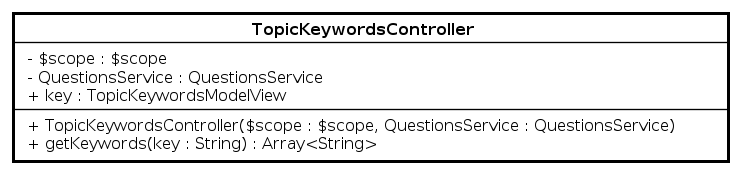
\includegraphics[scale=0.8]{UML/Classi/Front-End/QuizziPedia_Front-end_Controller_TopicKeywordsController.png}
	\caption{QuizziPedia::Front-End::Controllers::TopicKeywordsController}
\end{figure} \FloatBarrier
\begin{itemize}
	\item \textbf{Descrizione}: questa classe permette di gestire il recupero delle parole chiave di un questionario;
	\item \textbf{Utilizzo}: fornisce le funzionalità per il recupero delle parole chiave durante la creazione di un questionario;
	\item \textbf{Relazione con altre classi}:
	\begin{itemize}
		\item \textbf{IN \texttt{TopicKeywordsModelView}}: classe di tipo \textit{modelview\ped{G}} la cui istanziazione è contenuta all'interno della variabile di ambiente \$scope di \textit{Angular\ped{G}}. All'interno di essa sono presenti le variabili e i metodi necessari per il \textit{Two-Way Data-Binding\ped{G}} tra la \textit{view\ped{G}} \texttt{CreateQuestionnaireView} e il \textit{controller\ped{G}} \texttt{KeywordsController}; 
		\item \textbf{IN \texttt{QuestionsService}}: questa classe permette di ottenere domande esistenti e salvare nuove domande.
	\end{itemize}
	\item \textbf{Attributi}:
	\begin{itemize}
		\item \texttt{-} \texttt{\$scope: \$scope} \\
		Campo dati contenente un riferimento all'oggetto \$scope creato da \textit{Angular\ped{G}}, viene utilizzato come mezzo di comunicazione tra il \textit{controller\ped{G}} e la \textit{view\ped{G}}. Contiene gli oggetti che definiscono il \textit{model\ped{G}} dell'applicazione;
		\item \texttt{-} \texttt{QuestionsService: QuestionsService}\\ 
		Permette, tra le altre cose, di ottenere le parole chiave a partire da una stringa passata;
		\item \texttt{+} \texttt{key: TopicKeywordsModelView} \\
		Oggetto di tipo \texttt{CreateQuestionnaireView}. All'interno di esso sono presenti le variabili e i metodi necessari per il \textit{Two-Way Data-Binding\ped{G}} tra la \textit{directive\ped{G}} \texttt{TopicKeywor-\\dsDirective} e il \textit{controller\ped{G}} \texttt{TopicKeywordsController}.
	\end{itemize}
	\item \textbf{Metodi}:
	\begin{itemize}
		\item \texttt{+} \texttt{TopicKeywordsController(\$scope: \$scope, QuestionsService:\\ QuestionsService)} \\Metodo costruttore della classe. \\
		\textbf{Parametri}:
		\begin{itemize}
			\item \texttt{\$scope: \$scope} \\
			Parametro contenente un riferimento all'oggetto \$scope creato da \textit{Angular\ped{G}}. Viene utilizzato come mezzo di comunicazione tra il \textit{controller\ped{G}} e la \textit{view\ped{G}}. Contiene gli oggetti che definiscono il \textit{viewmodel\ped{G}} e il \textit{model\ped{G}} dell'applicazione;
			\item \texttt{-} \texttt{QuestionsService: QuestionsService}\\ 
			Permette, tra le altre cose, di ottenere le parole chiave a partire da una stringa passata.
		\end{itemize}
		\item \texttt{+} \texttt{getKeywords(key: String): Array<String>}	 \\ Metodo che ritorna le parole chiave data una una stringa di ricerca. \\
	\textbf{Parametri}:
	\begin{itemize}
		\item \texttt{key: String}: parametro che identifica la stringa con la quale cercare le keywords. 
	\end{itemize}
		\end{itemize}
\end{itemize}